\documentclass[11pt]{article}

\usepackage[a4paper]{geometry}
\usepackage{url}
\usepackage{enumitem}
\usepackage{amsthm}
\usepackage{graphicx}
\usepackage{float}
\usepackage{amssymb}

\theoremstyle{definition}
\newtheorem{exmp}{Example}[section]

\author{Laurens Vijnck}
\title{\textsc{Similar Items: Plagiarism Detection}}
\date{}

\begin{document}
	\maketitle
	
\section{Introduction}

The effort of establishing plagiarism is a prevalent application of detecting similar items. The ultimate goal of this project is to implement a data-parallel pipeline that performs plagiarism detection on code submissions. Concretely, the pipeline operates on a directory that contains coding submissions of students collected over the last few years. Each of these submissions is housed in a separate file that contains python source code. For privacy considerations, the submissions were anonymized. The desired output of the pipeline are the sets of submissions that have been identified as fraudulent.

As discussed in the lectures, the process of detecting similar items is rather costly. Techniques, such as \emph{Local Sensitive Hashing}, have been developed to the end of minimizing the required amount of work. Despite these techniques, performing similar item detection on a single machine can still be a time consuming process. We are interested in reducing the overall processing time of the procedure, specifically through \emph{parallelization}.

\section{Deliverables}

Due to the scope of this project, the project consists of two separate deliverables. The deadlines for these assignments are scheduled on 22/10/2019 12:00 and 13/11/2019 23:59 respectively. For each deliverable, hand in an .zip archive that contains the report and your code source files if applicable. Resort to the following naming convention:

\begin{verbatim}
	similar_items_G{group_number}_{lastname_student_1}_{lastname_student_2}.zip
\end{verbatim}

Concerning the reports, submit a \emph{single} file in .pdf format that specifies the following information in the header:

\begin{enumerate}[label=\textbf{\arabic*}.]
	\item Number of the group,
	\item Names of \emph{each} member of the group, and
	\item Student number of \emph{each} member of the group.
\end{enumerate}

Similar to the archive, using the following naming convention for the report. Note that, submissions that do not follow the aforementioned guidelines will \emph{not} be graded.

\begin{verbatim}
	report_G{group_number}_{lastname_student_1}_{lastname_student_2}.pdf
\end{verbatim}

\subsection{Initial Analysis}

First, perform a complete analysis of the assignment. It is advised to not implement anything at this stage. The deliverable of the analysis is a report that documents the approach to the problem. Moreover, elaborate on the issues you expect to encounter during implementation. The report should discuss \emph{at least} the following topics:

\begin{enumerate}[label=\textbf{\arabic*}.]
	\item How can we establish plagiarism in python source files? Keep in mind that students often tend to change solely the names of variables and functions within the code.
	
	\item Explain how Minhash signatures can be computed in a MapReduce environment and argue the correctness of your approach. Describe in detail how hashes are computed.
	
	\item Present the end-to-end architecture of the pipeline, preferably by means of a visualization. Draw specific attention to the input and output of each of the MapReduce stages involved. Clearly indicate the key used during reduce phases and describe the logic of non-trivial map operations.
\end{enumerate}

The intended use of this document is to guide you during implementation. It is therefore paramount that each step in the pipeline is thoroughly described. Refer to Example~\ref{ex:pipeline} for an example of the expected level of detail.

\begin{exmp}\label{ex:pipeline} Consider an arbitrary collection of input documents, where documents are augmented with author information. Assume for the sake of simplicity that documents have a single author. We are interested in implementing a custom version of the word-count pipeline. Specifically, when an author uses a specific word in multiple documents, it is accounted solely once in the final output. The end-to-end architecture of the pipeline is visualized by Figure~\ref{fig:example}.

\begin{figure}[]
\centering
	\makebox[\textwidth][c]{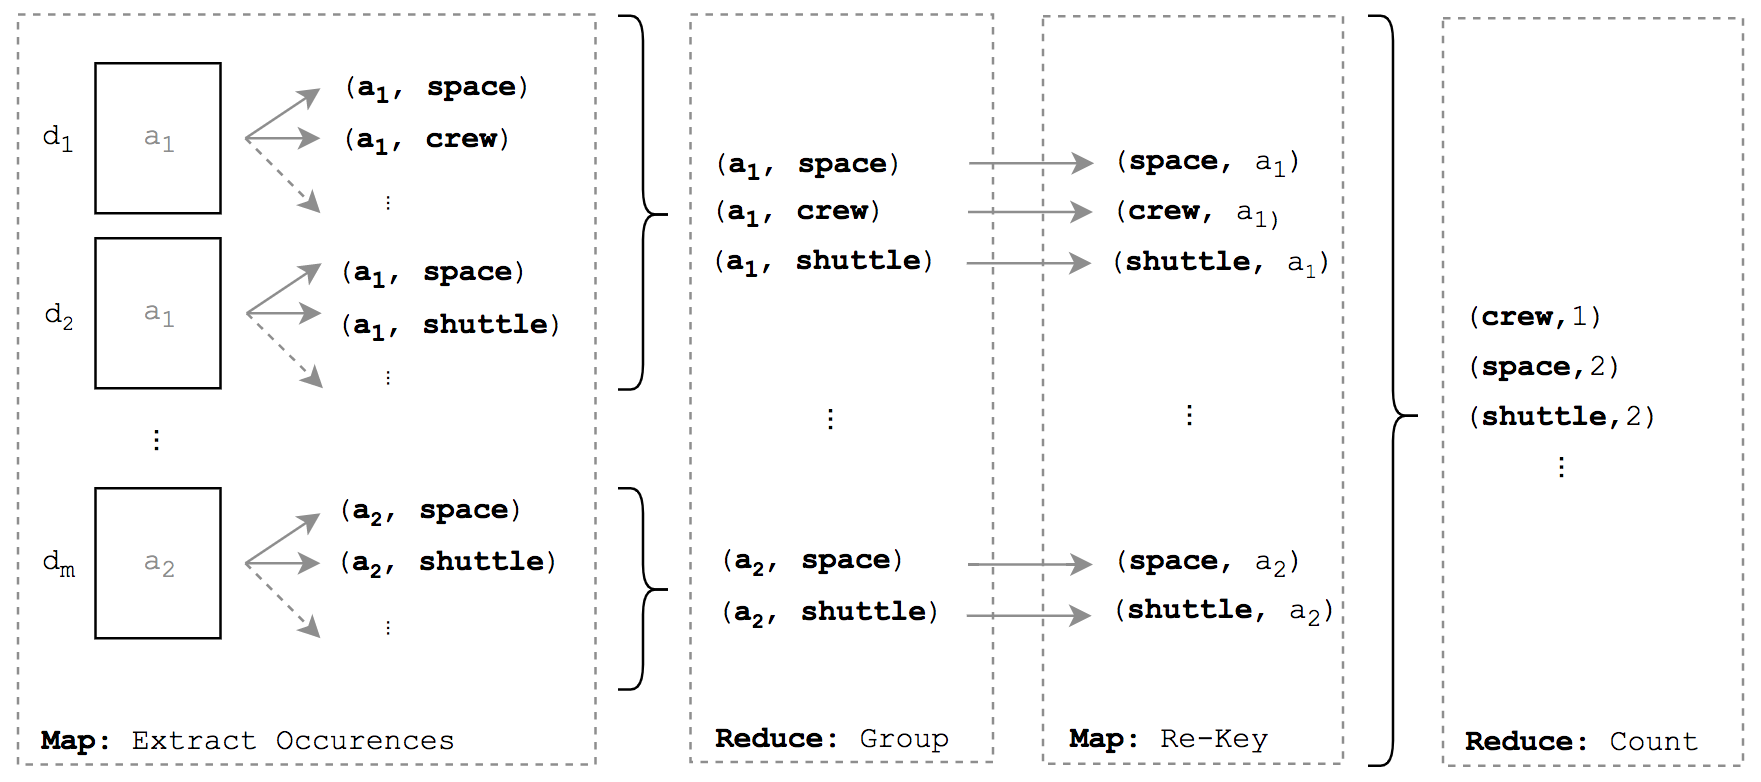
\includegraphics[width=1.2\textwidth]{example.png}}
	\caption{End-to-end word count pipeline with author deduplication.}
	\label{fig:example}
\end{figure}

The initial map stage considers each input document and extracts the contained words. It produces $(a, w)$ pairs, specifying that author $a$ used word $w$. The key of these elements is determined by both $a$ and $w$. This map step may produce multiple output elements per input document. Moreover, each document can be processed in parallel as there are no dependencies implied. The first reduce step is responsible for deduplicating words from the same author, it does so by grouping the output elements of the map phase according to their key. Hereafter, a one-to-one transformation is applied to alter the key of the incoming elements $(a, w)$ to $w$. The reduce step counts the total number of elements with a common key, thereby yielding a number of $(w, {count})$ pairs. The maximum amount of parallelism in the reduce phase is bounded by the number of unique words, that is, each key can be handled by a different instance. \hfill $\qed$
\end{exmp}

\subsection{Pipeline Implementation}

The second phase of this project involves an implementation of the pipeline in Apache Beam. Apache Beam\footnote{\url{https://beam.apache.org}} is a programming model for big data pipelines wherein pipelines are expressed as a sequence of logical transformations on input collections. Apache Beam comes with a very broad landscape of supporting execution engines, also referred to as runners. Popular runners are, among others, Apache Flink, Apache Spark, and Google Cloud Dataflow. Pipelines written in Beam are portable across runners in the sense that a pipeline has to be written once, and can be run anywhere desired. Moreover, the framework comes with a direct runner that allows quick iteration and prototyping. After handing in the initial reports, each group will be granted access to the Google Cloud Platform to develop their pipeline. The Google Cloud Platform offers a fully-managed solution for executing Beam pipelines.

Apache Beam is an open-source initiative that is under continuous development. While the runners are maintained by independent organizations, the functionality of the Beam model is not limited to the lowest common denominator thereof. Rather, the project attempts to incentivize the various runners to implement the latest standards into their execution engines.

The feedback session of 23/10/2019 will feature an introduction to Beam. For more information on how to build and test pipelines within the framework, resort to the Apache Beam Programming Guide\footnote{https://beam.apache.org/documentation/programming-guide/}.

\clearpage

\subsubsection{Final report}

Together with the pipeline implementation, hand in a report that discusses the following elements:

\begin{enumerate}[label=\textbf{\arabic*}.]
	\item Explain how your final implementation differs from the one presented in the initial analysis. Elaborate on the computation of the Minhash signatures and argue the correctness of your approach.
		
	\item Present the final architecture of the pipeline, preferably by means of a visualization. Draw specific attention to the input and output of each of the MapReduce stages involved. Clearly indicate the key used during reduce phases and describe the logic of non-trivial map operations.
	
	\item Discuss the results produced by your implementation, describe potential improvements and issues encountered along the way.
\end{enumerate}


\end{document}
